\subsection{THE A{[}X{]}-MODULE ASSOCIATED WITH AN A-MODULE ENDOMORPHISM}

Let M be an A-module and u an endomorphism of M. Consider the polynomial ring A{[}X{]} in one indeterminate X over A. For every polynomial \(p \in A[X]\) and all \(x \in M\) , we write

\[
p. x = p (u) (x).\tag{43}
\]

As \((pq)(u) = p(y) \circ q(u)\) for two polynomials p, q of A{[}X{]}, and A{[}X{]}-module structure is thus defined on M; the set M, with this structure, will be denoted by \(M_{u}\) ; the A-module structure given on M is obtained by restricting the ring of operators of \(M_{u}\) to A. Note that the submodules of \(M_{u}\) are just the submodules of M which are stable under u.

As the mapping \((p, x) \mapsto p \cdot x\) of \(\mathbf{A}[\mathbf{X}] \times \mathbf{M}\) into \(\mathbf{M}\) is A-bilinear, it defines canonically an A-linear mapping \(\phi: \mathbf{A}[\mathbf{X}] \otimes_{\mathbf{A}} \mathbf{M} \to \mathbf{M}\) such that

\[
\phi (p \otimes x) = p. x = p (u) (x).\tag{44}
\]

On the other hand, A{[}X{]} \(\otimes_{\mathbf{A}}\) M has canonically an A{[}X{]}-module structure (II, § 5, no. 1); we shall denote this A{[}X{]}-module by M{[}X{]}; the mapping \(\phi: \mathrm{M}[\mathrm{X}] \to \mathrm{M}_u\) is A{[}X{]}-linear since, for \(p, q\) in A{[}X{]} and \(x \in \mathbf{M}\) ,

\[
\phi (q (p \otimes x)) = \phi ((q p) \otimes x) = (q p). x = q (u) (p (u) (x)) = q. \phi (p \otimes x).
\]

Moreover, \(u\) is an A{[}X{]}-endomorphism of \(\mathbf{M}_u\) , for

\[
u (p. x) = u (p (u) (x)) = (u p (x)) (x) = p. u (x).
\]

Finally, an A{[}X{]}-endomorphism \(\bar{u}\) of M{[}X{]} is defined by writing (II, § 5, no. 1)

\[
\bar {u} (p \otimes x) = p \otimes u (x).\tag{45}
\]

Moreover it follows from formulae (44) and (45) that that A{[}X{]}-linear mappings u, \(\bar{u}\) and \(\phi\) are related by the relation

\[
\phi \circ \bar {u} = u \circ \phi .\tag{46}
\]

Let \(\psi\) denote the A{[}X{]}-endomorphism \(\mathbf{X} - \bar{\boldsymbol{u}}\) of M{[}X{]}, so that \(\psi(p \otimes x) = (\mathrm{X}p) \otimes x - p \otimes u(x)\) . We have the following proposition:

PROPOSITION 18. The sequence of A{[}X{]}-homomorphisms

\[
\mathbf {M} [ \mathbf {X} ] \stackrel {\psi} {\longrightarrow} \mathbf {M} [ \mathbf {X} ] \stackrel {\phi} {\longrightarrow} \mathbf {M} _ {u} \longrightarrow 0\tag{47}
\]

is exact.

As \(\phi(1 \otimes x) = x\) for all \(x \in \mathbf{M}\) , clearly \(\phi\) is surjective; on the other hand,

\[
\phi (\mathbf {X} (p \otimes x)) = \mathbf {X}. \phi (p \otimes x) = u (\phi (p \otimes x)),
\]

in other words, \(\phi \circ \mathbf{X} = u \circ \phi = \phi \circ \bar{u}\) by (46); this proves that \(\phi \circ \psi = 0\) . It remains to verify that \(\operatorname{Ker} \phi \subset \operatorname{Im} \psi\) . For this note that, since the monomials \(\mathbf{X}^k\) ( \(k \geqslant 0\) ) form a basis of the A-module \(\mathbf{A}[\mathbf{X}]\) , every element \(z \in \mathbf{M}[\mathbf{X}]\) can be written uniquely in the form \(z = \sum_k \mathbf{X}^k \otimes x_k\) , where \((x_k)\) is a family of elements of \(\mathbf{M}\) , of finite support. If \(z \in \operatorname{Ker} \phi\) , then \(\phi(z) = \sum_k u^k(x_k) = 0\) and we can write

\[
z = \sum_ {k} \left(\mathrm{X} ^ {k} \otimes x _ {k} - 1 \otimes u ^ {k} (x _ {k})\right) = \sum_ {k} \left(\mathrm{X} ^ {k} - \bar {u} ^ {k}\right) (1 \otimes x _ {k}).
\]

But as the A{[}X{]}-endomorphisms X and \(\bar{u}\) of M{[}X{]} are permutable, then

\(X^{k}-\bar{u}^{k}=(X-\bar{u})\circ\left(\sum_{j=0}^{k-1}X^{j}\bar{u}^{k-j-1}\right)\) which proves that there exists a \(y\in M[X]\) such that \(z=\psi(y)\) .

Now let \(\mathbf{M}'\) be another A-module and \(u'\) an endomorphism of \(\mathbf{M}'\) ; let \(\mathbf{M}_{u'}^{\prime}\) , \(\phi', \bar{u}', \psi'\) be the module and mapping obtained from \(\mathbf{M}'\) and \(u'\) as \(\mathbf{M}_u\) , \(\phi, \bar{u}, \psi\) are obtained from \(\mathbf{M}\) and \(u\) . Then:

PROPOSITION 19. For a mapping \(g\) of \(\mathbf{M}\) into \(\mathbf{M}'\) to be an \(\mathrm{A}[\mathrm{X}]\) -homomorphism of \(\mathbf{M}_u\) into \(\mathbf{M}_u'\) , it is necessary and sufficient that \(g\) be an A-homomorphism of \(\mathbf{M}\) into \(\mathbf{M}'\) such that \(g \circ u = u' \circ g\) . When this is so, if \(\bar{g}\) is the \(\mathrm{A}[\mathrm{X}]\) -homomorphism of \(\mathbf{M}[\mathrm{X}]\) into \(\mathbf{M}'[\mathrm{X}]\) equal to \(1_{\mathbf{A}[X]} \otimes g\) (II, § 5, no. 1), the diagram

\begin{enumerate}
\def\labelenumi{(\arabic{enumi})}
\setcounter{enumi}{47}
\tightlist
\item
\end{enumerate}

\pandocbounded{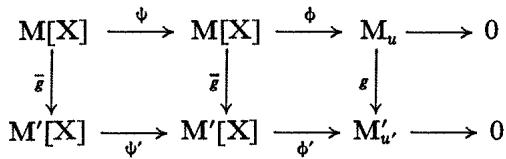
\includegraphics[keepaspectratio]{images/part004_f53e3a23.jpg}}

is commutative.

The condition \(g \circ u = u' \circ g\) is obviously necessary by (43) for \(g\) to be an A{[}X{]}-homomorphism; it is sufficient, for it implies by induction that \(g \circ u^n = u'^n \circ g\) for every integer \(n > 0\) . On the other hand, for all \(x \in M\) and all \(p \in A[X]\) ,

\[
\phi^ {\prime} (\bar {g} (p \otimes x)) = \phi^ {\prime} (p \otimes g (x)) = p (u ^ {\prime}) (g (x)) = g (p (u) (x)) = g (\phi (p \otimes x))
\]

and

\[
\bar {u} ^ {\prime} (\bar {g} (\boldsymbol {p} \otimes x)) = \bar {u} ^ {\prime} (\boldsymbol {p} \otimes g (x)) = \boldsymbol {p} \otimes u ^ {\prime} (g (x)) = \boldsymbol {p} \otimes g (u (x)) = \bar {g} (\bar {u} (\boldsymbol {p} \otimes x))
\]

which proves the commutativity of diagram (48).

